\documentclass[11pt,]{article}
\usepackage[left=1in,top=1in,right=1in,bottom=1in]{geometry}
\newcommand*{\authorfont}{\fontfamily{phv}\selectfont}
\usepackage[]{mathpazo}


  \usepackage[T1]{fontenc}
  \usepackage[utf8]{inputenc}



\usepackage{abstract}
\renewcommand{\abstractname}{}    % clear the title
\renewcommand{\absnamepos}{empty} % originally center

\renewenvironment{abstract}
 {{%
    \setlength{\leftmargin}{0mm}
    \setlength{\rightmargin}{\leftmargin}%
  }%
  \relax}
 {\endlist}

\makeatletter
\def\@maketitle{%
  \newpage
%  \null
%  \vskip 2em%
%  \begin{center}%
  \let \footnote \thanks
    {\fontsize{18}{20}\selectfont\raggedright  \setlength{\parindent}{0pt} \@title \par}%
}
%\fi
\makeatother




\setcounter{secnumdepth}{3}


\usepackage{graphicx,grffile}
\makeatletter
\def\maxwidth{\ifdim\Gin@nat@width>\linewidth\linewidth\else\Gin@nat@width\fi}
\def\maxheight{\ifdim\Gin@nat@height>\textheight\textheight\else\Gin@nat@height\fi}
\makeatother
% Scale images if necessary, so that they will not overflow the page
% margins by default, and it is still possible to overwrite the defaults
% using explicit options in \includegraphics[width, height, ...]{}
\setkeys{Gin}{width=\maxwidth,height=\maxheight,keepaspectratio}

\title{Mi playa\\
Subtítulo\\
Subtítulo  }



\author{\Large Ana Hilda Valera Arias\vspace{0.05in} \newline\normalsize\emph{Estudiante, Universidad Autónoma de Santo Domingo (UASD)}  }


\date{}

\usepackage{titlesec}

\titleformat*{\section}{\normalsize\bfseries}
\titleformat*{\subsection}{\normalsize\itshape}
\titleformat*{\subsubsection}{\normalsize\itshape}
\titleformat*{\paragraph}{\normalsize\itshape}
\titleformat*{\subparagraph}{\normalsize\itshape}

\titlespacing{\section}
{0pt}{36pt}{0pt}
\titlespacing{\subsection}
{0pt}{36pt}{0pt}
\titlespacing{\subsubsection}
{0pt}{36pt}{0pt}





\newtheorem{hypothesis}{Hypothesis}
\usepackage{setspace}

\makeatletter
\@ifpackageloaded{hyperref}{}{%
\ifxetex
  \PassOptionsToPackage{hyphens}{url}\usepackage[setpagesize=false, % page size defined by xetex
              unicode=false, % unicode breaks when used with xetex
              xetex]{hyperref}
\else
  \PassOptionsToPackage{hyphens}{url}\usepackage[unicode=true]{hyperref}
\fi
}

\@ifpackageloaded{color}{
    \PassOptionsToPackage{usenames,dvipsnames}{color}
}{%
    \usepackage[usenames,dvipsnames]{color}
}
\makeatother
\hypersetup{breaklinks=true,
            bookmarks=true,
            pdfauthor={Ana Hilda Valera Arias (Estudiante, Universidad Autónoma de Santo Domingo (UASD))},
             pdfkeywords = {palabra clave 1, palabra clave 2},  
            pdftitle={Mi playa\\
Subtítulo\\
Subtítulo},
            colorlinks=true,
            citecolor=blue,
            urlcolor=blue,
            linkcolor=magenta,
            pdfborder={0 0 0}}
\urlstyle{same}  % don't use monospace font for urls

% set default figure placement to htbp
\makeatletter
\def\fps@figure{htbp}
\makeatother

\usepackage{pdflscape} \newcommand{\blandscape}{\begin{landscape}}
\newcommand{\elandscape}{\end{landscape}}


% add tightlist ----------
\providecommand{\tightlist}{%
\setlength{\itemsep}{0pt}\setlength{\parskip}{0pt}}

\begin{document}
	
% \pagenumbering{arabic}% resets `page` counter to 1 
%
% \maketitle

{% \usefont{T1}{pnc}{m}{n}
\setlength{\parindent}{0pt}
\thispagestyle{plain}
{\fontsize{18}{20}\selectfont\raggedright 
\maketitle  % title \par  

}

{
   \vskip 13.5pt\relax \normalsize\fontsize{11}{12} 
\textbf{\authorfont Ana Hilda Valera Arias} \hskip 15pt \emph{\small Estudiante, Universidad Autónoma de Santo Domingo (UASD)}   

}

}








\begin{abstract}

    \hbox{\vrule height .2pt width 39.14pc}

    \vskip 8.5pt % \small 

\noindent Mi resumen


\vskip 8.5pt \noindent \emph{Keywords}: palabra clave 1, palabra clave 2 \par

    \hbox{\vrule height .2pt width 39.14pc}



\end{abstract}


\vskip 6.5pt


\noindent  \section{Introducción}\label{introducciuxf3n}

El mar constituye un elemento fundamental del conjunto de elementos de
la superficie terrestre capaz de generar cambios en las líneas de
costas, sean estas en una isla o continente. De acuerdo con Suárez de
Vivero (1999), el termino costa se puede aludir a la franja de tierra
que bordea el mar o a la zona de contacto entre el medio marino y el
medio terrestre. Teniendo en cuenta que la línea de costa puede variar
en un instante, por el paso de los años por la dinámica litoral o por
causa de fenomenos naturales, que pueden traer como posible concecuencia
la erosión o regresión de la costa.

Para Kokot (2004), la erosión costera es el resultado de un exceso de
remoción de sedimentos respecto del aporte suministrado al área en un
determinado periodo. La misma abarca la emersión y sumersión de
sedimentos en las orillas del mar o la playa, lo que mantiene en
constante movimiento el límite exacto de un verdadero perfil de costa.
Numerosos autores se han dedicado al estudio del análisis de cambio de
perfil de costa, usando como fuentes imágenes satelitales o fotografías
áereas históricas de la zona de estudio, además de hacer observaciones y
mediciones por un periodo de tiempo determinado que puedan dar respuesta
a dicho cambio o proceso; como es el caso de (Hernández Santana, Ortiz
Pérez, Méndez Linares, \& Gama Campillo, 2008).

La costa como unidad geomorfológica se mantiene en constante estado de
evolución. La importancia de conocer hacia dónde se desplaza más y que
forma ésta va adquiriendo, permite diferenciar el tipo de costa que, de
acuerdo con Codignotto (1997), pueden dividirse en: costa en
progradación, costa estacionaria y costa en retrogradación. Del mismo
modo, el autor hace énfasis en la importancia de comprender los factores
que iniciden en este proceso y las causas que lo producen.

De acuerdo con Aliotta, Spagnuolo, \& Farinati (2009), las rocas o beach
rock son formaciones sedimentológicas comunes que evidencian un proceso
erosivo del litoral, los cuales se dieron lugar en un ambiente
geoquímico que enmarcó un periodo de evolución continuo que pudo abarcar
varias etapas del tiempo geológico. Dónde en tal proceso la arena pudo
ser compactada por medio de cemento carbonático y al pasar varias épocas
posiblemete afloraron. En la isla de Santo Domingo las formaciones
arrecifales o rocas de playas datan del Neógeno y el periodo
cuaternario. Ejemplo según (\emph{Mapa de recursos minerales de la
república dominicana a escala 1}, n.d.), la Fm. Isabela del pleistoceno;
formación carbonatada arrecifal, rica en corales de tallas variables.
Aflora bajo la forma de diferentes relieves, formando arrecifes en
escalera descendiendo hacia el mar.

El litoral costero de la zona sur del país se caracteriza por pequeños
acantilados, playas de origen aluvial y dunas extensas (Abreu, 1999),
además, mareas con oleajes extremos típico del mar caribe. No obstante,
la ecología actúa como componente categorico en el microclima de una
zona, resultado de la diversidad que ésta puede aportar. Por tal motivo,
el interés de conocer el tipo de vegetación. Razón de que estos, sobre
la arena son preciso para la conservación de los sedimentos a
concecuencia de la erosión del viento y la lluvia.

Según (Cámara Artigas, 1997), los litorales de la isla, se caracterizan
por tener flores propias de la especie árboreas o herbáceas como la
coccoloba\_uvífera (uvas de playas), (ver figura \ref{coccoloba}) y la
IPomoea\_Pescaprea (ver figura \ref{ipomoea}). De igual modo la
vegetación cercanas a aguas dulce o salada suele llamarse bosques de
manglares, estos suelen encontrarse en algunas dunas costeras de la
parte sur del país, principalmente en las riveras y desembocaduras de
cuencas lacustre. Conforme Polanía \& Nat (1998), estos tipos de bosques
son asociaciones vegetales que prosperan en las costas tropicales y
subtropicales del mundo. Pero en la isla de Santo Domingo existe una
tipología diferente en dichos espacios costeros.

La playa de Najayo se encuentra ubicada en la sección del mismo nombre,
perteneciente al municipio San Gregorio de Nigua, provincia San
Cristobal, al Sur de la Republica Dominicana. Fisiográficamente, se
ubica en la llanura costera del Caribe, en las coordenadas aproximadas
18º17'40" latitud Norte y 70º06'02" longitud Oeste. De acuerdo al mapa
geológico de la isla de Santo Domingo (Abad de los Santos, 2007--2010),
se estima que la formación del relieve costero de Najayo data de la era
Cenozoica periodo Cuaternario entre las época Eoceno-Mioceno, el mismo
está compuesto por arena y gravas bioclásticas formando el cordón
litoral, además de conglomerado, gravas, arenas de fondo de valle,
calizas arrecifales, calciruditas y calcarenitas (ver figura
\ref{mapageo50k}).

\begin{figure}
\centering
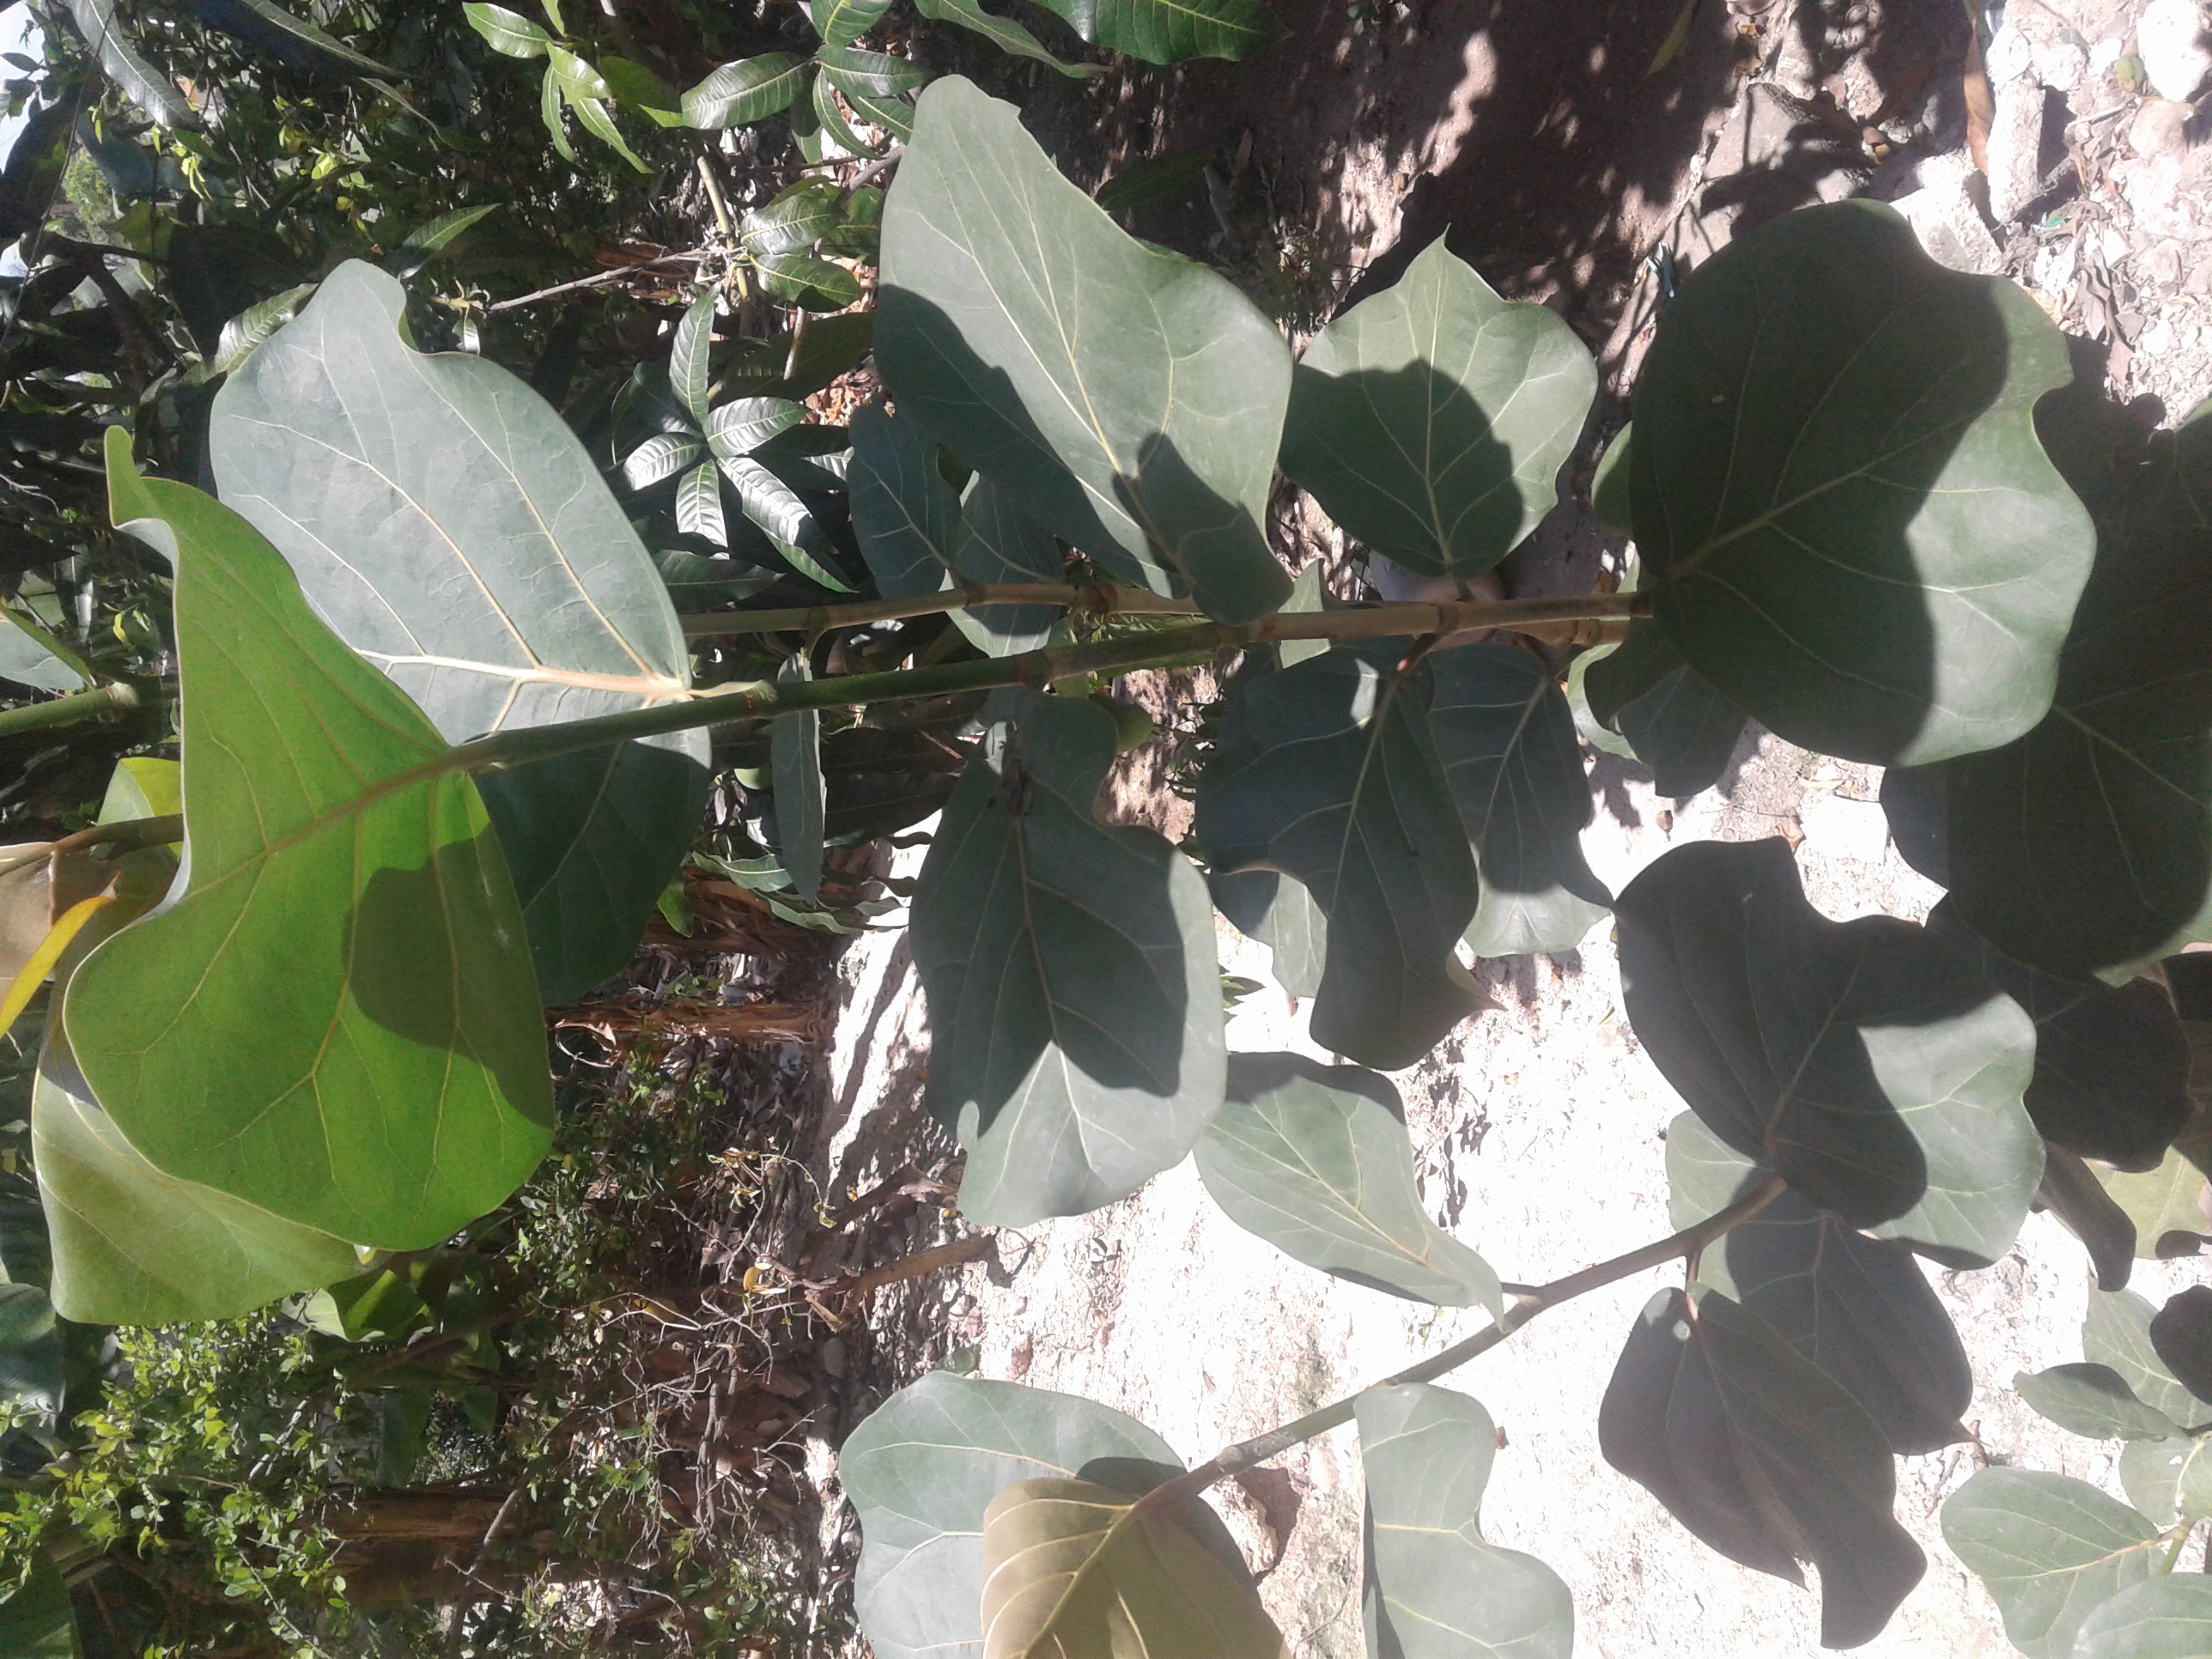
\includegraphics{coccoloba_uvifera.jpg}
\caption{Vegetación dunas de playa\label{coccoloba}}
\end{figure}

\begin{figure}
\centering
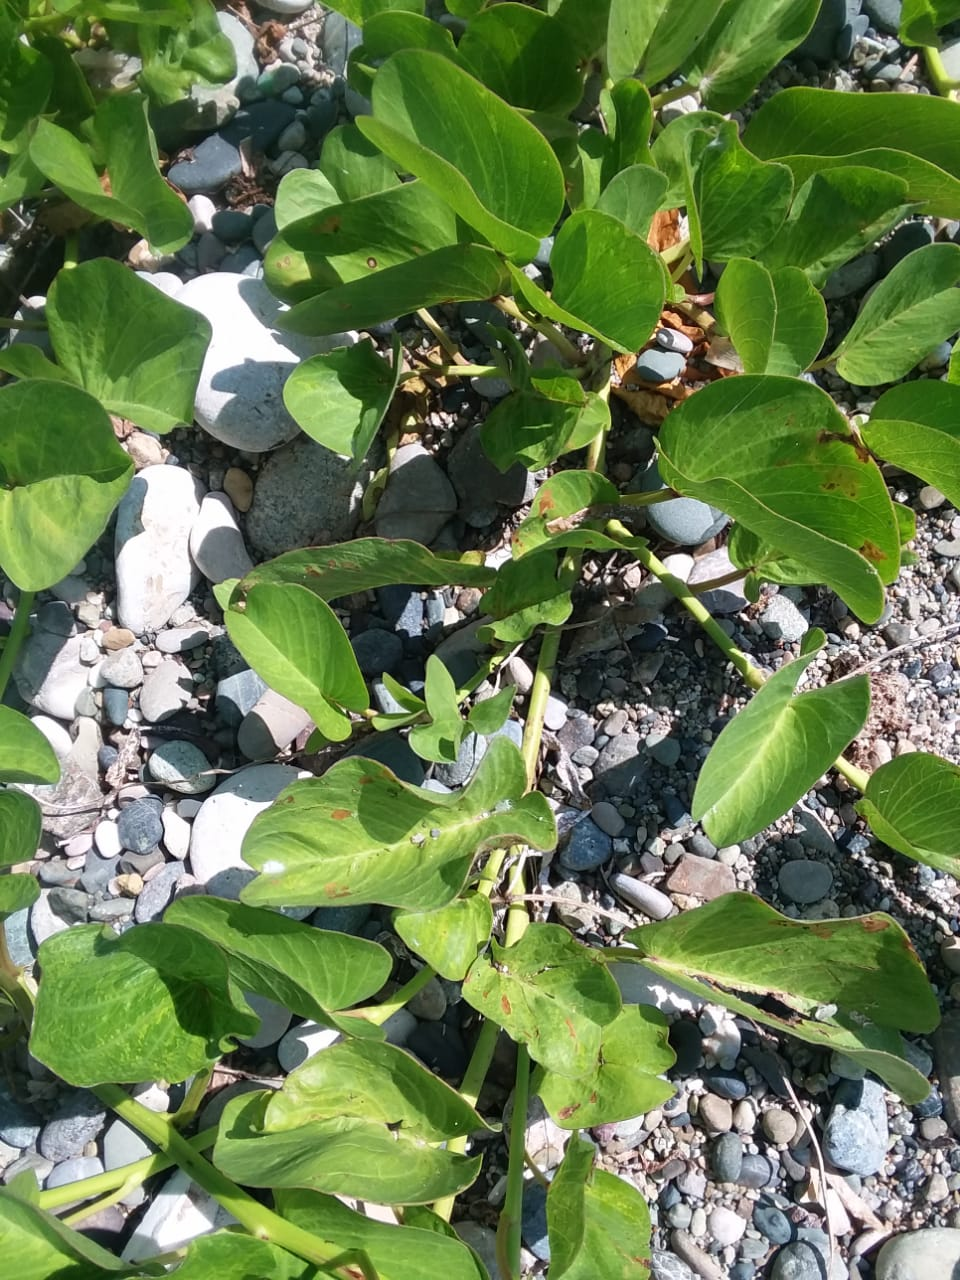
\includegraphics{Ipomoea_Pescaprea.jpg}
\caption{Vegetación riveras de playa-río\label{ipomoea}}
\end{figure}

\begin{figure}
\centering
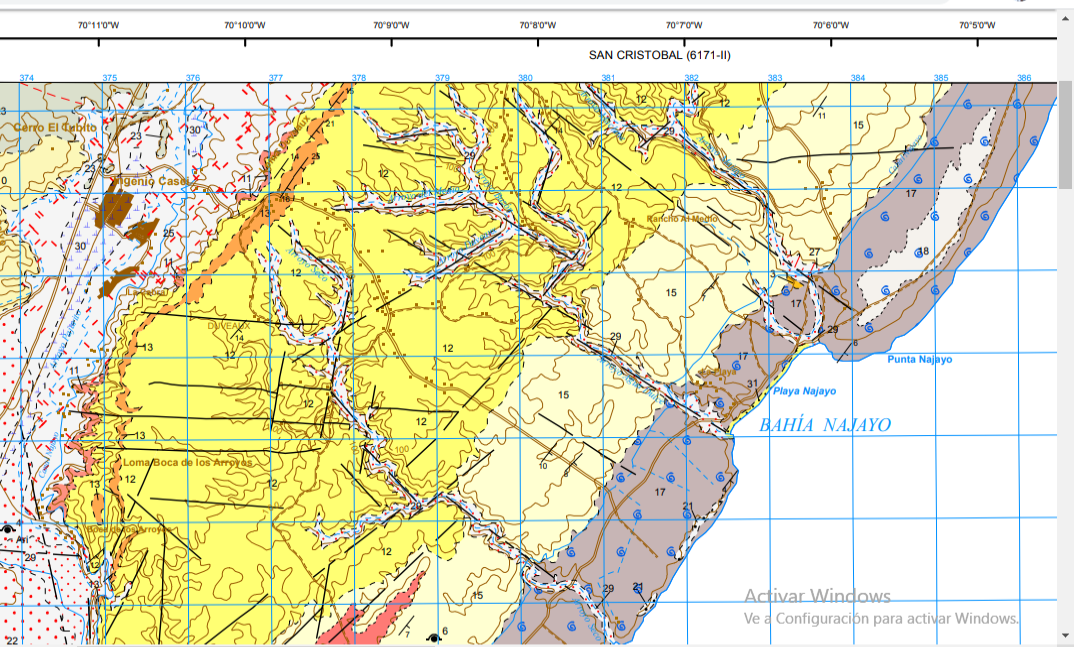
\includegraphics{mapa_bahia_najayo.png}
\caption{Mapa geológico escala 1:50,000 (hoja Nizao)\label{mapageo50k}}
\end{figure}

\ldots

\section{Metodología}\label{metodologuxeda}

Para el análisis de cambio de línea de costa en la playa los pescadores
sección Playa Najayo se tomó como referencia para estudio,imágenes
satélitales de Landsat 8 de los años (1973,1978,1979,1981 y 1982), en
las cuales se delimitó tales líneas con el programa Qgis. Además de
colectar arenas y gravas en varios puntos de la costa. También por medio
de la aplicación ODK Collection se llenó un formulario en el campo y se
tomó las coordenadas geograficas de cada punto. Asimismo, se hizo vuelo
de Dron en la costa para obtener información reciente de la actual
línea.

Cada punto seleccionado para la recaudación de muestra fueron
identificado por área con respecto al mar o la playa (Berma y Dunas de
Playa), además de su ubicación mediante puntos cardinales.

\ldots

\section{Resultados}\label{resultados}

\ldots

\section{Discusión}\label{discusiuxf3n}

\section{Agradecimientos}\label{agradecimientos}

\section{Información de soporte}\label{informaciuxf3n-de-soporte}

\ldots

\section{\texorpdfstring{\emph{Script}
reproducible}{Script reproducible}}\label{script-reproducible}

\ldots

\section*{Referencias}\label{referencias}
\addcontentsline{toc}{section}{Referencias}

\hypertarget{refs}{}
\hypertarget{ref-abad2007mapageonizao}{}
Abad de los Santos, M. (. (2007--2010). \emph{Mapa Geológico de la
República Dominicana a escala 1:50.000 de la hoja n 6170-I (Nizao) y
Memoria correspondiente}. Santo Domingo: Proyecto 1B de Cartografía
Geotemática de la República Dominicana. Programa SYSMIN. Servicio
Geológico Nacional.

\hypertarget{ref-abreu1999impacto}{}
Abreu, L. (1999). Impacto del turismo en el litoral de dominicana.
\emph{Revista Geográfica}, 167--182.

\hypertarget{ref-aliotta2009origen}{}
Aliotta, S., Spagnuolo, J. O., \& Farinati, E. A. (2009). Origen de una
roca de playa en la región costera de bahía blanca, argentina.
\emph{Pesquisas Em Geociências}, \emph{36}(1), 107--116.

\hypertarget{ref-camara1997republica}{}
Cámara Artigas, R. (1997). \emph{República dominicana: Dinámica del
medio físico en la región caribe (geografía física, sabanas y litoral)
aportación al conocimiento de la tropicalidad insular}.

\hypertarget{ref-codignotto1997geomorfologia}{}
Codignotto, J. (1997). \emph{Geomorfología y dinámica costera}.

\hypertarget{ref-hernandez2008morfodinamica}{}
Hernández Santana, J. R., Ortiz Pérez, M. A., Méndez Linares, A. P., \&
Gama Campillo, L. (2008). Morfodinámica de la línea de costa del estado
de tabasco, méxico: Tendencias desde la segunda mitad del siglo xx hasta
el presente. \emph{Investigaciones Geográficas}, (65), 7--21.

\hypertarget{ref-kokot2004erosion}{}
Kokot, R. R. (2004). \emph{Erosión en la costa patagónica por cambio
climático}.

\hypertarget{ref-diaz2007memoria}{}
\emph{Mapa de recursos minerales de la república dominicana a escala 1:
100.000 de la hojan 6271 (santo domingo) y memoria correspondiente}.
(n.d.).

\hypertarget{ref-polania1998manejo}{}
Polanía, J., \& Nat, R. (1998). Manejo de ecosistemas de manglar.
\emph{Memorias Del Curso Manejo de Ecosistemas de Manglar Y Arrecifes de
Coral. Bogotá}, 153--168.

\hypertarget{ref-suarez1999delimitacion}{}
Suárez de Vivero, J. L. (1999). Delimitación y definición del espacio
litoral. \emph{Jornadas Sobre El Litoral de Almería: Caracterización,
Ordenación Y Gestión de Un Espacio Geográfico Celebradas En Almería, 20
a 24 de Mayo de 1997. Pag: 13-23}.




\newpage
\singlespacing 
\end{document}
